
%%%%%%%%%%%%%%%%%%%%%%%%%%%%%%%%%%%%%%%%%%%%%%%%%%%%%%%%%%%%%%%%%%%%%%%%%%%%%%%%%%
\chapter{Organization and Management}
\label{v1ch:org-mgmt}

\section{LBNF}
\subsection{LBNF Organization and Management}

\subsubsection{Overview}

The LBNF Project is charged by Fermilab and DOE to design and construct conventional and technical facilities to support DUNE. LBNF works closely with DUNE through several coordinating groups to ensure scientific direction and coordination to execute the LBNF Project. LBNF also works closely with SURF management to coordinate design and construction for the facilities for the DUNE Far Detector. 

LBNF consists of two major subprojects coordinated by a central Project Office located at Fermilab: Far Site Facilities and Near Site Facilities. Each of the L2 Projects consists of major L3 Projects as shown in the WBS structure in section \fixme{xx}.

The Project Team consists of people from Fermilab, CERN, SDSTA, and BNL. The Team includes Project Office members and L2 and L3 Project leaders who manage the Project. The team is assembled by the Project Director. The Project team to WBS Level 3 of the WBS is shown in Figure~\ref{fig:lbnf-org}.  Line management for environment, safety, and health and quality assurance flows through the Project Director. 

Through their delegated authority and in consultation with major stakeholders, the L2 Project Managers appoint the WBS Level 3 Managers, and also determine which of their lower tier managers will be Control Account Managers (CAMs) for the Project WBS. L2 and L3 Project Managers are directly responsible for generating and maintaining the cost estimate, schedule, and resource requirements for their Projects and for meeting the goals of their Project within the accepted baseline cost and schedule. 

The design and construction of LBNF is supported by other laboratories and consultants/contractors, which provide scientific, engineering, and technical expertise. A full description of LBNF Project Management is contained in the LBNF Project Management Plan \fixme{[ref]}.

\begin{cdrfigure}[LBNF Organization to WBS L3]{lbnf-org}{LBNF Organization to WBS L3; note that the WBS numbers reflect the pre-CD1 WBS}
  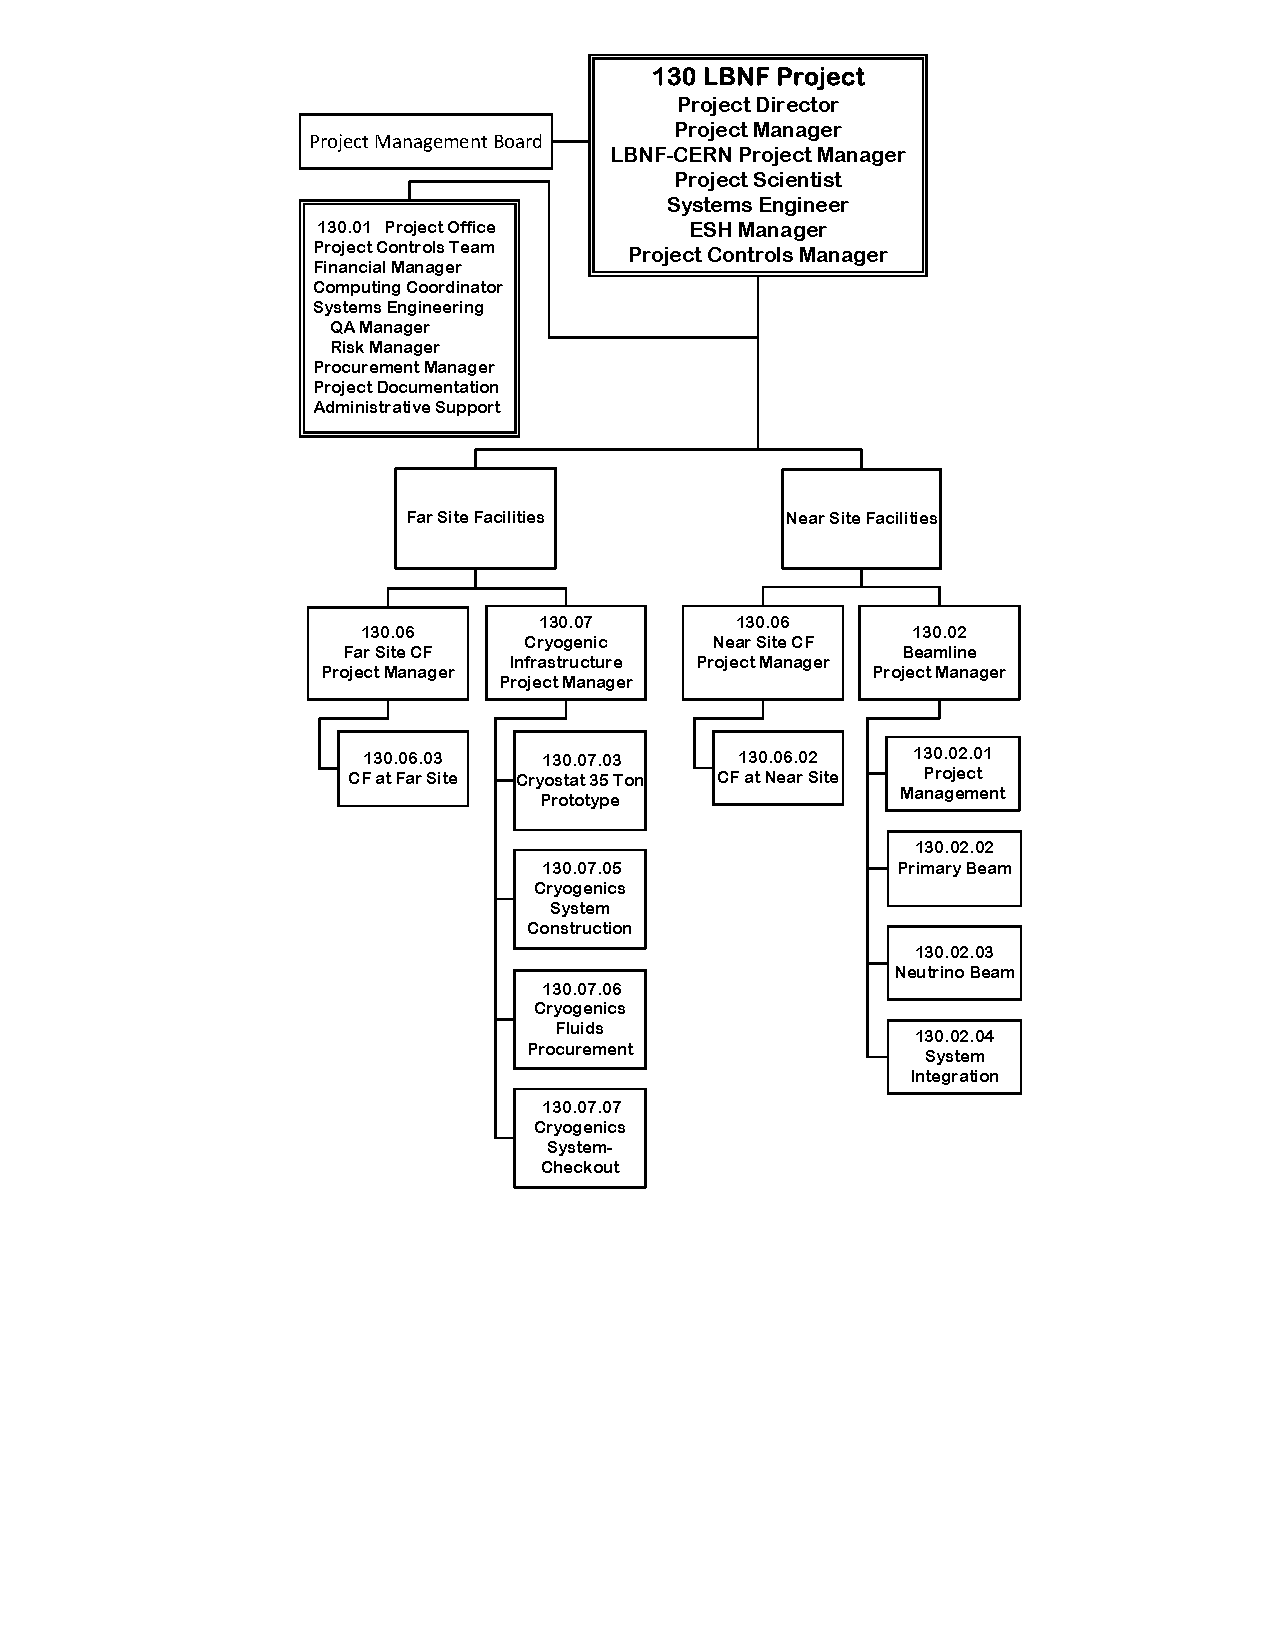
\includegraphics[width=0.8\textwidth]{lbnf-org-to-level3}
\end{cdrfigure}

\subsubsection{South Dakota Science and Technology Authority and SURF}

LBNF plans to construct facilities at SURF to house the DUNE Far Detector. This facility is owned by the state of South Dakota and managed by the South Dakota Science and Technology Authority (SDSTA). 

Current SURF activities include operations necessary to to allow safe access to the 4850L for the existing and under-development science experiments. DOE is presently funding SDSTA ongoing operations through Lawrence Berkeley National Laboratory (LBNL) and its SURF Operations Office through FY16; this is expected to change to funding through Fermilab starting in FY17. 

The LBNF Far Site Facilities Manager is also an employee of SDSTA and is contracted to Fermilab to provide management and coordination of the Far Site Facilities CF and Cryo Infrastrastrucre. The LBNF Project also contracts directly with SDSTA to provide the management and design of LBNF Conventional Facilities at SURF; consruction for the CF will be directly contracted from Fermilab. Coordination with SDSTA and the LBNF Project is necessary to ensure efficient operations at SURF while meeting LBNF requirements. This will be facilitated with an agreement being developed between SDSTA and Fermilab regarding the LBNF Project [new reference], that defines responsibilities and methods of working together during the LBNF Project design and construction. A separate agreement will be written for LBNF Operations. 

\subsubsection{CERN}

The European Organization for Nuclear Research (CERN) will participate in the LBNF Project by providing cryogenic facilities and equipment to support the Far Detector and some technical components for the Beamline. As a key Facilities partner, CERN will provide the design and production, as well as coordinate with others in LBNF for the installation for identified deliverables. CERN engineers and scientists will participate in LBNF as assigned managers for specific scope as outlined in the sections below. 

Details of the agreements with CERN will be contained in  \fixme{[name the agreements here]}.  

\subsection{LBNF Organization}

\subsubsection{At Fermilab }
The LBNF Project line organization is headed by the LBNF Project Director who is also the Fermilab Deputy Director for LBNF and reports to the Fermilab Director. The Project Director heads two divisions that align with the LBNF L2 Projects: Far Site Facilities and Near Site Facilities. At the time of CD-1 Refresh Review, this organization is transitioning into existence and is expected to be in place in Fall 2015. Personnel who are working more than half time on the project are expected to be in these divisions while others may be matrixed part-time as required from other Fermilab Divisions/Sections/Centers or may work on LBNF as requested. Fermilab D/S/C Heads work with the L1 and L2 Project Managers to supply resources on an annual basis. 

\subsubsection{At SDSTA}
SDSTA assigns engineers and others as required to work on specific tasks required for LBNF. This is listed in the resource-loaded schedule as contracted work from Fermilab for Far Site CF activities. 

\subsubsection{At CERN}
CERN and Fermilab are developing a common cryogenics team for LBNF as well as other liquid argon engineering activities. CERN assigns engineers and other staff as required to accomplish LBNF cryo infrastructure tasks. 

\subsubsection{Coordination within LBNF}

\textbf{Project Management Board:} LBNF uses a Project Management Board to provide formal advice to the Project Director on matters of importance for the LBNF Project as a whole. Such matters include (but are not limited to) those that:
\begin{itemize}
\item have significant technical, cost or schedule impact on the Project
\item have impacts on more than one L2 Project
\item affect the management systems for the Project
\item have impacts on or result from impact from other Projects on which the LBNF is dependent
\item result from external reviews or reviews called by the PD
\end{itemize}
The Management Board serves as the
\begin{itemize}
\item LBNF Change Control Board, as described in the Configuration Management Plan \fixme{[ref]}
\item Risk Management Board, as described in the Fermilab Risk Management Plan  \fixme{[ref]}
\end{itemize}

\textbf{Beamline Technical Board:} The role of the LBNF Beamline Technical Board is to provide recommendations and advice to the Beamline Project Manager on important technical decisions that affect the design and construction of the Beamline. The members of the Technical Board must have knowledge of the Project objectives and priorities in order to perform this function. The Beamline Project Manager chairs the Beam TB. The Beamline Project Engineer is the Scientific Secretary of the Board and co-chairs the Beam TB as needed. 

\textbf{FSCF Neutrino Cavity Advisory Board:} The FSCF Project has engaged three international experts in hard rock underground construction to advise it periodically through the design and construction process regarding excavation at SURF. The board meets at the request of the FSCF-PM, generally on site to discuss specific technical issues. The board produces a report with its findings and conclusions for project information and action. 

\subsubsection{Work Breakdown Structure}
The LBNF WBS defines the scope of the work. All changes to the WBS must be approved by the LBNF Project Manager prior to implementation. At the time of CD-1-Refresh, the LBNF WBS is in transition. Both the current and the post CD-1-R WBS is shown in Figure~\ref{fig:lbnf-wbs} to demonstrate how the scope will map from one WBS to the other. 

\begin{cdrfigure}[LBNF Work Breakdown Structure to WBS Level 3]{lbnf-wbs}{LBNF Work Breakdown Structure to WBS Level 3}
  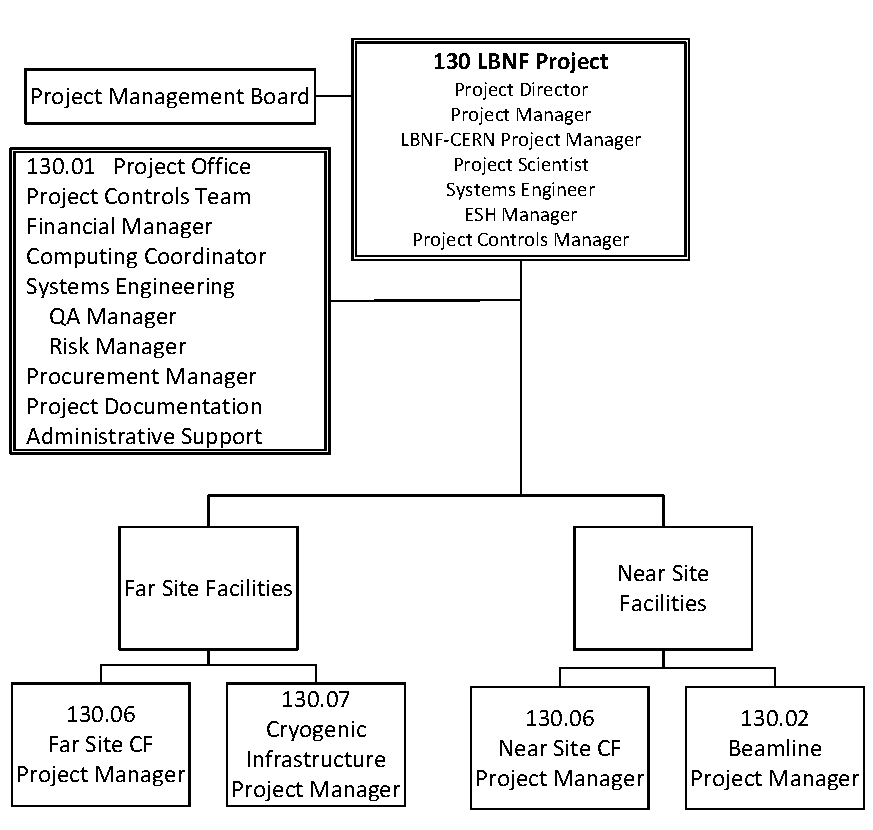
\includegraphics[width=0.8\textwidth]{lbnf-wbs-to-level3}
\end{cdrfigure}



%%%%%%%%%%%%%%%%%%%%%%%%%%%%%%%%%%%%%%%%%%%%%%%%%%%%%
\section{DUNE Organization and Management}

%\subsection{DUNE Science Collaboration and Project Office}
%The international DUNE experiment is managed through two tightly-coupled structures: the DUNE Science Collaboration and the DUNE Project Office.  The DUNE Science Collaboration is responsible for the scientific and experimental strategy, while the DUNE Project Office is responsible for the implementation of this strategy within the context of the available international resources.
%
%%An overview of the organization of the two entities is given in the following:
%%\begin{itemize}
%%\item {\bf DUNE Science Collaboration}: 
%\subsection{DUNE Science Collaboration}

The DUNE Collaboration brings together the members of the international science community 
interested in participating in the DUNE experiment.  The Collaboration defines the scientific goals of the experiment and subsequently 
the requirements on the experimental facilities needed to achieve these goals.  The Collaboration also provides the scientific and 
technical effort required for the design and construction of the DUNE detectors, operation of the experiment, and analysis of the 
collected data. There are four main elements in the DUNE organizational structure:  
{\it the DUNE collaboration}, comprised of the General Assembly of the collaboration and the DUNE Institute Board;     
{\it DUNE management}, the two co-spokespersons, the Technical Coordinator (TC), the Resource Coordinator (RC), who along
  with the IB chair and five other members of the collaboration form the DUNE Executive Committee (EC); 
{\it the DUNE Project Office (PO)}; and
{\it the DUNE Science Team}, led by the Physics and Software/Computing coordinators. 

The main responsibilities of the different roles are summarised below:
\begin{itemize}
  \item {\bf The DUNE General Assembly} is composed of all members of the collaboration, it is consulted on major strategic decisions 
    through open plenary sessions at collaboration meetings and is informed through regular collaboration phone calls;
  \item {\bf The DUNE Institutional Board} represents the institutes of the collaboration. It is composed of one representative from each 
    of the member institutions and has responsibility for Collaboration governance.  The IB has final authority over Collaboration 
    membership issues and defines requirements for inclusion of individuals within the DUNE authorship list. The IB is also responsible    
    for establishing and monitoring the process through which the co-spokespeople are selected to serve as leaders of the collaboration.   
  \item {\bf The DUNE co-spokespersons} are accountable to the collaboration. They 
    are responsible for the day-to-day running of the collaboration and for representing the collaboration to Fermilab, funding 
    agencies and the broader scientific community.
  \item{\bf  The DUNE Executive Committee (EC)} is chaired by the longest serving co-spokesperson and is the primary 
    decision-making body of the collaboration. Membership of the EC includes the co-spokespeople, DUNE Project Office leaders, IB 
    chair, and five additional Collaboration members (three elected IB representatives and two additional members selected by the co-
    spokespeople). The EC will work by consensus. In the cases where consensus cannot be reached, 
    the authority lies with the spokespeople. If the co-spokespeople disagree, the TC will arbitrate.
  \item {\bf The Technical Coordinator (TC)} reports to the spokespersons and the Fermilab director. 
     The TC acts as the project director 
    and is responsible for the implementation of the scientific and technical strategy of the collaboration through the DUNE project office.
    The TC is also responsible for the management of the DOE contributions to the DUNE project.  
     The Technical Coordinator prepares and chairs the meetings of the Technical Board of the experiment collaboration.
     \item{\bf The Technical Board (TB)} discusses and approves the technical planning for all subsystems of the DUNE detector;
       \item {\bf The Resource Coordinator (RC)} reports to the spokespersons and the Fermilab director. The RC
    The Resources Coordinator is responsible for coordinating the financial planning and other
resources issues of the collaboration. The Resource Coordinator is responsible in particular for
the management of the common resources of the Collaboration (common fund).
The Resources Coordinator prepares and chairs the meetings of the Finance Board (internal) of
the experiment collaboration. The Resources Coordinator is responsible for the
preparation of the Memoranda of Understanding of the Collaboration.
    \item{\bf The Finance Board (FB)} is responsible for dealing with matters related to
the costs and resources of the Collaboration, evaluation of the contributions, relations with the
funding agencies and all administrative matters.  
    \item{\bf The DUNE Science Team} is led by the physics coordinator and the software/computing coordinator and is responsible for the management of the DUNE scientific WGs;
    \item{\bf The DUNE Project Office (PO)} provides the project management for the design, construction, installation, and commissioning of the DUNE near and far detectors. DUNE will be run as an international project matching DOE requirements. This will imply maintaining a full cost and schedule for the entire project, from which the DOE-funded portion can be extracted and monitored in a manner that satisfies DOE reporting requirements. The DUNE Project Office will have direct control over DOE project funds and any common fund collected from the U.S. and international stakeholders. International contributions to DUNE will be in the form of deliverables as defined in formal Memoranda of Understanding (MOU). These contributions will be tracked through detailed sub-project milestone. The entire Project (including international contributions) will be subject to the DOE critical decision process incorporating a CD-2 approval of its baseline cost and schedule and a CD-3 approval for moving forward with construction.  
    \item{\bf The DUNE Technical WGs} The organization of the technical working groups of the DUNE collaboration is the responsibility of the L2 managers in the DUNE project.
\end{itemize}


\fixme{add Work Breakdown Structure ?}


\fixme{add Project Schedule}



